\documentclass[12pt]{extarticle}
\usepackage{geometry}
\usepackage{graphicx}
\usepackage{listings}
\usepackage{hyperref}

\geometry{
	a4paper,
	top = 2cm,
	left = 2.5cm,
	bottom = 2cm,
	right = 2.5cm,
}
\author{Pierciro Caliandro (matr 0299815)}
\title{Report dell'homework \#1}
\date{}

\begin{document}
\maketitle
%\tableofcontents
\section{Scopo del documento e definizione dell'obiettivo}
Il seguente documento mostra i passi seguiti per l'analisi del file \textbf{hw1.exe}, riportando quella che è stata la metodologia adottata durante l'attività di reverse code engineering.\\
Prima di partire con l'analisi del codice e le attività di reversing è stato definito un obiettivo, in modo da avere ben chiaro quale è lo scopo del reversing.\\ In questo caso, lo scopo prefissato è quello di \textbf{individuare le strutture di dati principali utilizzate all'interno del programma} e di cercare in generale di carpire quante più informazioni possibili sul programma.\\ Come tool per analizzare il codice del file eseguibile oggetto di studio è stato utilizzato Ghidra.
\section{Ricerca del main}
Il primo passo dell'analisi è stato quello di cercare la funzione main, per farlo si è scelto di affidarsi alla visualizzazione data dal function call tree. Partendo dall'entry point, sono state espanse tutte le chiamate a funzione, fino all'ultimo livello, come mostrato nella figura seguente\\\\
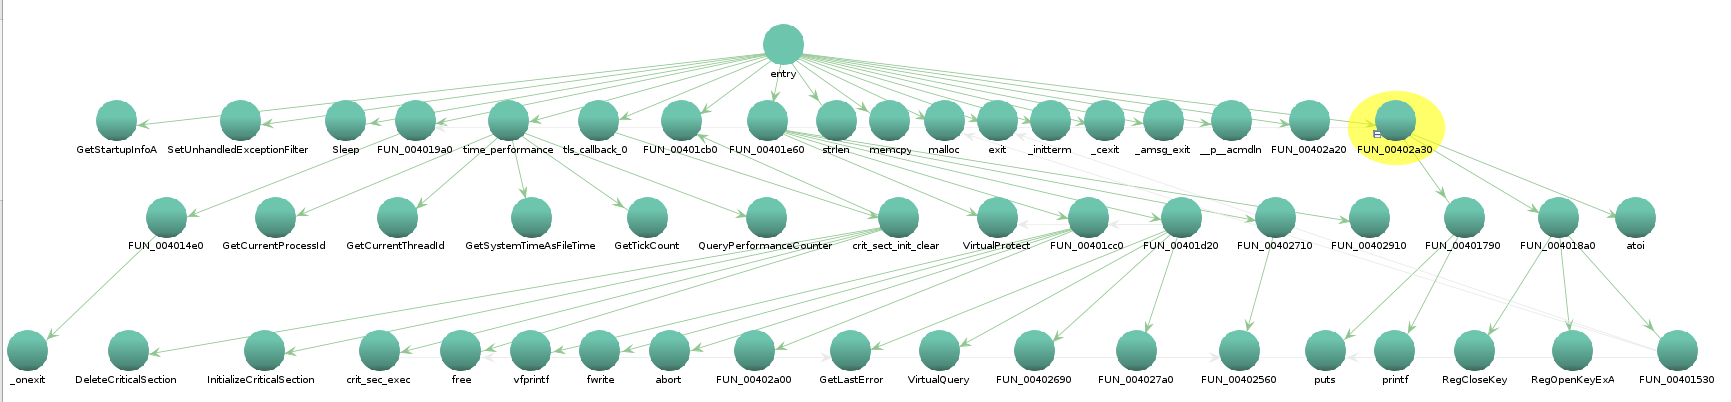
\includegraphics[scale=0.3]{immagini/hw1_main}\\\\
Si può notare che ci sono delle chiamate a funzioni di libreria quali
\begin{itemize}
\item \textit{puts}
\item \textit{printf}
\item \textit{atoi}
\end{itemize}
questo può portare a pensare che tali funzioni siano state invocate all'interno del codice per scelta del programmatore e quindi si è tentato di risalire l'albero al contrario per tenare di capire da quali funzioni partono le chiamate.\\
Ad esempio, la \textit{puts} e la \textit{printf} vengono chiamate dalla routine \textbf{FUN\_0040179}, a sua volta chiamata dalla \textbf{FUN\_00402a30} e proprio da quest'ultima viene chiamata la \textit{atoi}. Quindi, sembrerebbe che la funzione \textbf{FUN\_00402a30} sia una buona candidata ad essere la funzione \textbf{main} del programma.\\ 
Partendo dall'entry point, è stato analizzato cosa avviene prima della chiamata alla routine \textbf{FUN\_00402a30}, sia guardando il codice assembly che tramite il tool di decompilazione di Ghidra. Proprio nella seguente immagine viene riportato il codice prodotto dallo strumento di decompilazione di Ghidra\\\\
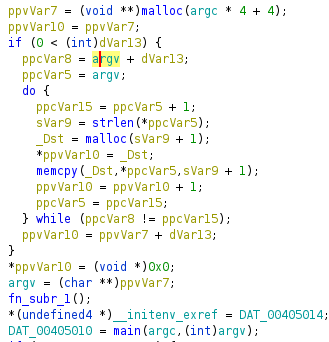
\includegraphics[scale=0.5]{immagini/pre-main}\\\\
Vi sono le seguenti istruzioni: 
\begin{itemize}
\item la variabile automatica \textsf{ppVar7} viene inizializzata con una \textbf{malloc}, castata a \textsf{void**}, ed il parametro della malloc è la variabile globale \textsf{DAT\_0040501c}, che viene moltiplicata per 4, per poi venire aggiunta a 4;
\item alla variabile automatica \textsf{ppVar10} viene associato il valore di \textsf{ppVar7};
\item all'interno di un ciclo do/while, viene
\begin{itemize}
\item associata alla variabile automatica \textsf{sVar9} il valore di ritorno della \textit{strlen}, chiamata usando come parametro la variabile dereferenziata \textsf{ppcVar5}, a cui fuori dal ciclo era stato associato il valore di \textsf{DAT\_00405018};
\item la variabile \textsf{\_Dst} viene allocata nello heap tramite chiamata alla \textbf{malloc}, allocando un numero di byte pari a \textsf{sVar9} + 1;
\item viene poi fatta una \textbf{memcpy} all'intero di \textsf{\_Dst} del valore puntato da \textsf{ppcVar5}, prima è stato associato a \textsf{ppvVar10} il valore di \textsf{\_Dst}, dopo averlo dereferenziato in quanto la variabile automatica \textsf{ppvVar10} è stata riconosciuta da Ghidra come di tipo \textsf{void **};
\end{itemize}
alla fine del ciclo, viene associato alla variabile globale \textsf{DAT\_00405018} il riferimento, castato a \textsf{char **} di \textsf{ppvVar7}, che a sua volta riferiva \textsf{ppvVar10}. Quindi, questo è l'argomento del main \textsf{char **argv}, mente l'argomento \textsf{int argc} risulta essere la variabile \textsf{DAT\_0040501c}. Infatti, questi vengono poi passati come parametri alla funzione \textbf{FUN\_00402a30}, dove però argv viene castato ad \textsf{int}.
\end{itemize}
Infine, è stata marcata come \textbf{main} la funzione che aveva label \textbf{FUN\_00402a30}, ed inoltre all'interno di Ghidra è stato cambiato il tipo del parametro argv a \textsf{char **}.\\ Successivamente, è stata svolta una analisi di cosa accade all'interno del main:
\begin{itemize}
\item c'è una chiamata ad una funzione che a sua volta invoca la \textbf{\_onexit()}, siccome sembrerebbe che tale routine sia auto-generata, si prosegue con l'analisi ignorandola;
\item viene verificato se il valore \textsf{argv[argc]} è pari a 0, se lo è si setta il valore di ritorno della funzione a 0, altrimenti si va avanti;
\item andando avanti, si verifica se il numero di parametri passati in argv è minore di 3, se lo è si impostano i valori di \textsf{argv[1]} ed \textsf{argv[2]} a 0, altrimenti si prosegue con le istruzioni;
\item a questo punto c'è quello che ha tutta l'aria di essere l'inizializzazione dei parametri da passare ad una funzione:
\begin{itemize}
\item si invoca la funzione \textbf{atoi}, passando come parametro il valore di argv[1], dopo di che si carica nel registro EDX una stringa esadecimale. Dal decompilatore possiamo vedere che il primo parametro della funzione viene castato a tipo HKEY e cercando nella documentazione di 	Windows è possibile scoprire che la stringa esadecimale messa in EDX, ovvero "0x80000002", corrisponde alla costante \textbf{HKEY\_LOCAL\_MACHINE}. Tale valore viene assegnato al primo dei parametri di input nel caso in cui il valore di argv[1] sia NULL, ovvero l'utente non abbia specificato alcun parametro a riga di comando per il programma;
\item anche per il secondo parametro di input si procede in modo simile, ovvero prima si verifica se il valore di \textsf{argv[2]} è diverso da NULL e nel caso non lo sia si setta il valore del secondo parametro uguale alla stringa \textbf{SYSTEM$\backslash\backslash$ControlSet001
$\backslash\backslash$Control};
\end{itemize}
\end{itemize}
A questo punto viene eseguita la chiamata a funzione passando i due parametri dallo stack, tale funzione è stata rinominata \textbf{fn\_reg\_open\_close\_key}.
\section{Apertura e chiusura del registry key}
All'interno della funzione \textbf{fn\_reg\_open\_close\_key} vengono inizializzate 5 variabili automatiche, per poi passare alla CALL della funzione di libreria \textbf{RegOpenKeyExA}. Dalla documentazione di Windows, è possibile scoprire cosa fa e quali parametri prende la funzione:
\begin{itemize}
\item la funzione apre uno specifico registry key, restituendo come valore di ritorno un \textsf{LSTATUS}, ovvero un codice di errore pari a 0 se la chiamata è andata a buon fine e diverso da 0 in caso di errore;
\item i parametri presi in input ed output sono i seguenti:
\begin{itemize}
\item[1)] [in] \textsf{HKEY hKey}: un handle ad un open registry key. Se non è stata specificata alcuna chiamata alle funzioni \textbf{RegCreateKeyEx} o \textbf{RegOpenKeyEx} il parametro può avere un valore di default, che in questo caso è \textbf{HKEY\_LOCAL\_MACHINE};
\item[2)] [in, optional] \textsf{LPCSTR lpSubKey}: il nome del registry subkey da aprire. Nella documentazione viene detto che se questo valore è nullo o punta ad una stringa vuota, nel parametro di output \textsf{phkResult} verrà messo lo stesso hKey handle ricevuto nel primo parametro;
\item[3)] [in] \textsf{DWORD  ulOptions}: opzioni da associare quando si apre il registry, in questo caso viene semplicemente impostato a 0;
\item[4)] [in] \textsf{REGSAM samDesired}, una maschera che specifica i privilegi di accesso alla chiave. Si usa in questo caso, nella funzione, la primitiva di default \textbf{KEY\_ALL\_ACCESS}, che è stato trovato sempre dalla documentazione ed associato alla maschera di bit mediante il comando "Equate" di Ghidra;
\item[5)] [out] \textsf{PHKEY  phkResult}: un puntatore che riceve l'handle alla chiave aperta
\end{itemize}
\end{itemize}
Dopo il ritorno della chiamata a \textbf{RegOpenKeyExA}, viene valutato il valore di ritorno:
\begin{itemize}
\item se è diverso da 0, c'è stato un errore e quindi la funzione salta all'epilogo, salvando in EAX il valore di ritorno, cioè NULL;
\item se è diverso da 0, viene utilizzato il valore ritornato nel parametro \textsf{phkResult}, ovvero l'handle al registry key, passandolo ad una funzione che è stata denominata come \textbf{key\_info\_retrieve}
\end{itemize}
Infine, viene chiuso il registry mediante la funzione di libreria \textbf{RegCloseKey}, che prende come unico parametro l'handle registry key aperto, e viene ritornato una variabile di tipo LPSTR *, che quindi potrebbe essere un puntatore ad una area di memoria che contiene il risultato della funzione \textbf{key\_info\_retrieve}. Come detto precedentemente, in caso di fallimenti viene restituito NULL.
\subsection{Enumerazione dei valori e delle sotto-chiavi associati alla chiave}
Nella funzione \textbf{key\_info\_retrieve}, vengono chiamate due malloc per allocare della memoria dinamica:
\begin{itemize}
\item la prima malloc alloca area nello heap per un totale di 52 byte;
\item si mette il risultato della prima malloc, e quindi il puntatore all'area di memoria appena allocata, all'interno del registro EBX;
\item si chiama una nuova malloc, stavolta allocando 260 byte;
\item il puntatore a questa nuova zona di memoria allocata si salve dentro la base del registro EBX, che quindi ora i primi 4 byte conterranno l'indirizzo di un buffer di 260 byte
\end{itemize} 
C'è poi l'inizializzazione di diverse variabili automatiche, tutte di tipo puntatore, che vengono passate alla funzione \textbf{RegQueryInfoKeyA}:
\begin{itemize}
\item la funzione restituisce informazioni relative allo specifico registry key. Anche in questo caso, il valore di ritorno è 0 in caso di successo o un valore negativo in caso di fallimento;
\item i parametri di input ed output sono i seguenti, tutti quanti inizializzati spiazzandosi all'interno di EBX, quindi usando le aree di memoria precedentemente allocate dalla malloc:
\begin{itemize}
\item[1)] [in] \textsf{HKEY hKey}: l'handle all'oper registry key, non è altro che il primo parametro passato alla funzione;
\item[2)] [out, optional] \textsf{LPSTR lpClass}: puntatore a un buffer che riceve la classe della chiave definita dall'utente. lpClass è proprio un pointer ai 260 byte allocati dalla seconda malloc, infatti viene impostato facendo una MOV del registro EAX nel 2° parametro della funzione;
\item[3)] [in, out, optional] \textsf{LPDWORD lpcchClass}: la size del buffer puntato da lpClass, espresso in caratteri, il puntatore si trova in EBX+4 e contiene proprio il valore 260;
\item[4)] [out, optional] \textsf{LPDWORD lpReserved}: parametro riservato che deve essere NULL, infatti viene settata la corrispondente variabile locale tramite una MOV di 0x0;
\item[5)] [out, optional] \textsf{LPDWORD lpcSubKeys}: un puntatore ad un parametro che riceve il numero di sotto-chiavi;
\item[6)] [out, optional] \textsf{LPDWORD lpcbMaxSubKeyLen}: puntatore ad una variabile che riceve la taglia della sotto-chiave col prefisso più lungo;
\item[7)] [out, optional] \textsf{LPDWORD lpcbMaxClassLen}: puntatore ad una variabile che riceve la taglia della stringa più lunga che specifica la classe di una subkey;
\item[8)] [out, optional] \textsf{LPDWORD lpcValues}: puntatore che riceve il numero di valori associati alla chiave;
\item[9)] [out, optional] \textsf{LPDWORD lpcbMaxValueNameLen}: puntatore che riceve la taglia del nome del valore più grande fra quelli associati alla chiave;
\item[10)] [out, optional] \textsf{LPDWORD lpcbMaxValueLen}: puntatore che riceve la taglia del più grande campo dati fra i valori della chiave;
\item[11)] [out, optional] \textsf{LPDWORD lpcbSecurityDescriptor}: puntatore che riceve la taglia del security descriptor associato alla chiave;
\item[12)] [out, optional] \textsf{PFILETIME lpftLastWriteTime}: puntatore ad una struttura di tipo FILETIME, che riceve l'ultima volta che è stata effettuata una scrittura 
\end{itemize}
\end{itemize}
Tutte quante le variabili automatiche, essendo di tipo puntatore, vengono allocate utilizzando EBX, in quanto dal codice assembly si vedono una serie di \textsf{MOV dword ptr}, quindi area di memoria dinamica. Siccome le locazioni di memoria di EBX vengono accedute ad indirizzi contigui, è ragionevole pensare che sia stata allocata una struttura dati nello heap, per contenere le informazioni di interesse che verranno poi ritornate al chiamante. I campi della struttura vengono acceduti per riferimento, siccome la funzione vuole tutti parametri di tipo puntatore.\\
In seguito alla chiamata, si verifica poi il valore di ritorno della funzione:
\begin{itemize}
\item se il valore è diverso da 0, si salta ad un label, che è stata rinominata \textbf{info\_key\_err\_label}, in cui si stampa a schermo un stringa che indica un errore mediante la funzione di libreria \textbf{puts}. Dopo di che, si salta ad una label di uscita, rinominata come \textbf{exit\_label\_1};
\item se il valore è 0, si mette in EDX il valore alla locazione di memoria EBX + 8, che contiene il parametro \textsf{lpcSubKeys}, ovvero il numero di sotto-chiavi associate alla chiave;
\item si verifica se il valore è maggiore di 0:  in caso in cui sia minore, si salta ad una label in cui si carica in EBX+44 il valore di EAX, in questo caso impostato a NULL e dopo di che si carica in EAX il puntatore all'area di memoria EBX+20, che sappiamo contenere il parametro \textsf{lpcValues}, ovvero il numero di valori associati alla chiave.
\end{itemize}
\subsubsection{Enumerazione delle sotto-chiavi}
Nella label dentro la quale viene svolta l'enumerazione delle sotto-chiavi, quindi il caso di \textsf{lpcSubKeys} $>$ 0, ci sono le seguenti operazioni di inizializzazione, tutte inferite dal codice assembly
\begin{itemize}
\item vengono allocati 16 byte con una malloc e messi nel registro EBP;
\item si esegue un'altra malloc, stavolta di un numero di byte pari al valore dato da \textsf{lpcbMaxSubKeyLen}, quindi si alloca spazio in modo da assere sicuri di poter contenere per intero il nome di qualunque valore venga letto;
\item il risultato della seconda malloc viene salvato ad indirizzo EBP+8;
\item viene messo EBP all'interno del registro EDI.
\end{itemize}
A questo punto si inizializzano i parametri di input da passare alla funzione \textbf{RegEnumKeyExA}
\begin{itemize}
\item la funzione va ad enumerare le sotto-chiavi di uno specifico registry key di Windows, avendo come valore di ritorno lo stesso delle due funzioni di libreria precedenti, ovvero un intero pari a 0 in caso di successo e negativo in caso di fallimento;
\item riassumendo i parametri di input ed output della funzione:
\begin{itemize}
\item[1)] [in] \textsf{HKEY hKey}: handle ad un open registy key, lo stesso usato nella chiamata predente;
\item[2)] [in] \textsf{DWORD dwIndex}: l'indice della subkey da trovare. Per la prima chiamata l'indice doverebbe essere 0, per poi venire incrementato di uno ogni volta. È possibile vedere dal modo in cui vengono settati i parametri sullo stack che tale indice è contenuto nel registro ESI, che viene infatti azzerato prima di entrare nella label e viene incrementato dopo la chiamata alla funzione. Inoltre, viene sempre confrontato col valore ad indirizzo EBX+8, che è proprio il numero totale di subkeys da cercare. Se il valore di ESI è inferiore a tale numero, si risalta alla label iniziale, quindi la scansione avviene all'interno di un loop, che Ghidra interpreta come un do/while;
\item[3)] [out] \textsf{LPSTR lpName}: puntatore ad un buffer che riceve il nome della sottochiave, incluso il byte nullo (terminatore di stringa);
\item[4)] [in, out] \textsf{LPDWORD lpcchName}: puntatore ad un parametro che indica la taglia del buffer \textsf{lpName}. Dal codice assembly si può vedere che tale valore viene sempre settato a \textsf{lpcbMaxSubKeyLen}, così da essere sicuri che il buffer avrà sempre abbastanza spazio per contenere il nome della sottochiave;
\item[5)] \textsf{LPDWORD lpReserved}: puntatore ad un area di memoria che deve essere impostato a NULL;
\item[6)] [in, out] \textsf{LPSTR lpClass}: puntatore ad un buffer che riceve la definizione utente della classe associata al valore;
\item[7)] [in, out, optional] \textsf{LPDWORD lpcchClass}: taglia del buffer puntato da \textsf{lpClass};
\item[8)] [out, optional]\textsf{PFILETIME lpftLastWriteTime}: puntatore ad una struttura di tipo FILETIME che riceve l'ultimo timestamp di scrittura associato alla chiave. Il parametro viene caricato in EDX accedendo allo stesso usato nella chiamata precedente, quindi lo stesso contenuto nella struct iniziale;
\end{itemize}
\end{itemize}
Al termine della chiamata, viene messo in EDI il puntatore all'area di memoria EBP + 4, per poi verificare se si torna all'interno del ciclo, confrontando l'indice contenuto nel registro ESI col valore di \textsf{lpcSubKeys}. Come si vede, appena vi è il rientro nel ciclo ed a seguito della prima malloc, viene messo in EAX+4 il valore di EDI e quindi in EBP+12 visto che l'istruzione in seguito è proprio una MOV di EAX in EBP+12.\\ Questo fa pensare che la struttura di dati usata all'interno di questo loop sia una lista collegata, dove viene ogni volta fatto puntare il nodo successivo al precedente. L'organizzazione del nodo della struttura viene riassunto nella seguente immagine:\\\\
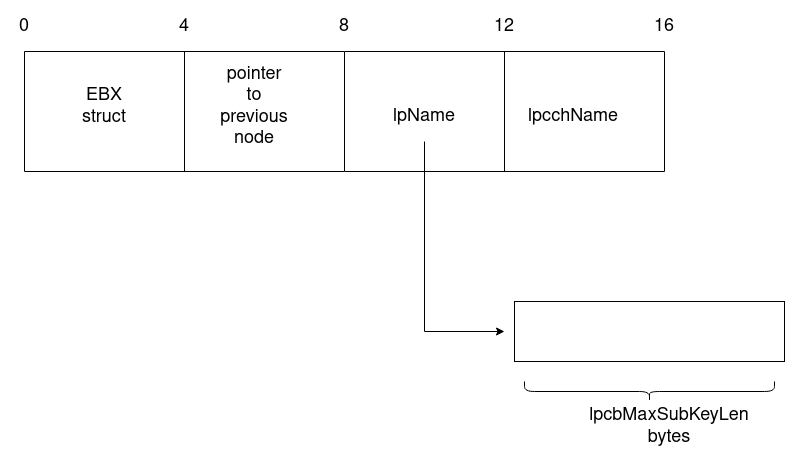
\includegraphics[scale=0.27]{immagini/struct_chiavi}
\\\\Completata l'enumerazione delle chiavi, il valore del registro ESI e quindi l'intera lista collegata viene salvato all'indirizzo EBX+44, per poi passare a verificare se ci sono dei valori da enumerare.
\subsubsection{Enumerazione dei valori}
Prima di partire con l'enumerazione dei valori, viene re-impostato il registro EDI a 0, così come anche ESI e viene caricato in EAX il valore puntato da EBX+20, ovvero \textsf{lpcValues}.\\ Viene quindi fatto un test su EAX per verificare se ci sono effettivamente dei valori da enumerare, in tal caso si salta alla label dentro cui avviene l'enumerazione. Nel caso in cui non ci fosse alcun valore associato alla chiave, si esce mettendo nella locazione di memoria ad indirizzo EBX+48 il valore di ESI, in questo caso NULL per poi tornare il controllo al chiamante.\\
Saltando alla label in cui si enumerano i valori, anche in questo caso consultando il decompilatore, si nota che Ghidra ha interpretato il ciclo in cui avviene questa operazione come un do/while, che va avanti usando come indice il registro EDI finché il valore di quest'ultimo non supera il valore dato da \textsf{lpcValues}, ovvero non sono stati letti tutti i valori associati alla chiave.\\ Anche qui come nel ciclo precedente, viene allocata della memoria dinamica mediante la malloc, in questo caso per 16660 byte. Anche qui, come è avvenuto per le due chiamate precedenti, i byte vengono usati per inizializzare i puntatori che verranno usati come parametri per la funzione di libreria \textbf{RegEnumValueA}:
\begin{itemize}
\item la funzione enumera i valori per lo specifico registry key, copiando per ogni chiamata un singolo nome del valore con il corrispettivo blocco dati, in base all'indice passato. Il valore di ritorno è sempre 0 se la funzione è andata a buon fine ed un valore negativo in caso di errore;
\item i parametri di input ed output sono riassunti di seguito:
\begin{itemize}
\item[1)] [in] \textsf{HKEY hKey}: handle ad un open registry key;
\item[2)] [in] \textsf{DWORD dwIndex}: indice del valore da recuperare;
\item[3)] [out] \textsf{LPSTR lpValueName}: puntatore ad un buffer che riceve il nome del valore, incluso il byte nullo;
\item[4)] [in, out] \textsf{LPDWORD lpcchValueName}: un puntatore che specifica la taglia del buffer che conterrà \textsf{lpValueName}, in caratteri;
\item[5)] \textsf{LPDWORD lpReserved}: puntatore NULL;
\item[6)] [out, optional] \textsf{LPDWORD lpType}: puntatore ad una variabile che riceve un codice che indica il tipo di dato salvato dallo specifico valore;
\item[7)] [out, optional] \textsf{LPBYTE lpData}: puntatore ad un buffer che riceve i dati associati al valore;
\item[8)] [in, out, optional] \textsf{LPDWORD lpcbData}: un puntatore ad una variabile che contiene la taglia del buffer puntato da \textsf{lpData}. Il valore di ritorno contiene il numero di byte scritti il lpData.
\end{itemize}
\end{itemize}
EDI è quindi il valore usato per \textsf{dwIndex} che all'interno di una label, che è stata denominata \textbf{cycle\_cond}
\begin{itemize}
\item viene incrementato sempre di uno, confrontato col valore presente alla locazione di memoria data da EBX + 20;
\item se risulta minore o uguale si salta ad una label dopo cui si esegue l'epilogo;
\item altrimenti, si ritorna all'inizializzazione dei parametri della funzione per una nuova chiamata della \textbf{RegEnumValueA}.
\end{itemize} 
Anche in questo caso, EBP viene salvato nel registro ESI che poi a sua volta all'interno del ciclo viene messo nell'indirizzo EAX+4, dopo la malloc, quindi questo di nuovo indica la possibilità che il programmatore abbia utilizzato una struttura dati che è una lista collegata dove il nodo corrente punta a quello precedente.\\
Scendendo nel dettaglio di come vengono inizializzati questi parametri di input, è possibile vedere che 
\begin{itemize}
\item i byte da 16656 a 16660 contengono il valore \textsf{lpcbData};
\item i byte da 16400 a 16656 vengono usati come buffer per \textsf{lpData};
\item alla base di EAX, viene caricato EBX;
\item i byte da 16396 a 16400 sono usati per il parametro \textsf{lpType};
\item i byte da 16392 a 16396 vengono invece usati per il puntatore al parametro \textsf{lpcchValueName}, che indica la taglia del buffer \textsf{lpValueName} che è di 16383 byte, escluso il terminatore di stringa;
\item ad indirizzo EBP + 8 viene messo il puntatore a \textsf{lpValueName}, dove il primo byte, cioè quello ad offset 8 (rispetto alla base EBP), viene impostato a 0 in quanto nel buffer deve essere compreso il terminatore di stringa;
\end{itemize}
Viene di seguito mostrata una figura che mostra l'organizzazione del singolo nodo:\\\\
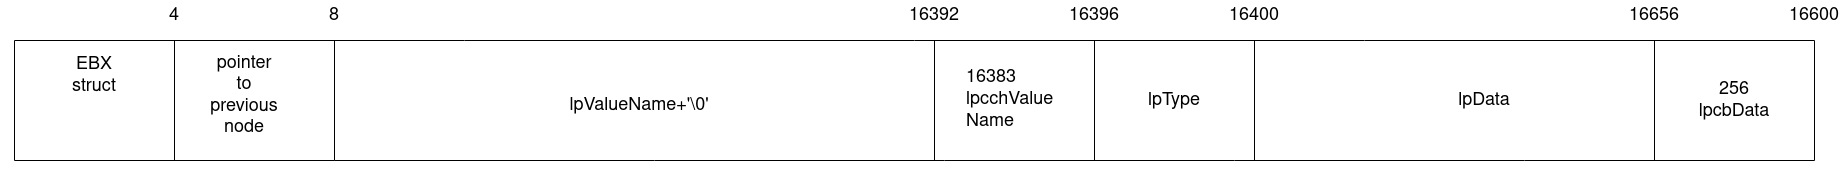
\includegraphics[scale=0.27]{immagini/struct_valori}\\\\
Una volta terminato il ciclo, viene messo il valore di ESI, quindi l'intera lista collegata, all'interno della cella di memoria ad indirizzo EBX+48, si esegue quindi il prologo e si restituisce il controllo alla funzione chiamante.\\\\ Di seguito, vengono riassunte le possibili strutture dati in C corrispondenti alle 3 individuate nell'analisi:\\
\begin{lstlisting}
struct subkey_node{
	struct key_info *infokey;
	struct key_node *previous;	
	LPSTR lpName;
	LPSTR lpcbMaxSubKeyLen;	
};
\end{lstlisting}
\begin{lstlisting}
struct value_node{
	struct key_info *infokey;
	struct value_node *previous;
	LPSTR lpValueName;
	DWORD lpcchValueName;
	DWORD lpType;
	BYTE lpData;
	DWORD lpcbData;
};
\end{lstlisting}
\begin{lstlisting}
struct key_info{
	LPSTR lpClass;
	DWORD lpcchClass;
	DWORD lpcSubKeys;
	DWORD lpcbMaxSubKeyLen;
	DWORD lpcbMaxClassLen;
	DWORD lpcValues;
	DWORD lpcbMaxValueNameLen;
	DWORD lpcbMaxValueLen;
	DWORD lpcbSecurityDescriptor;
	FILETIME lpftLastWriteTime;
	struct subkey_node * key_node_head;
	struct value_node *value_list_head;
};
\end{lstlisting}
Le strutture dati sono state inserite in Ghidra, in modo da facilitare la comprensione del codice prodotto dal decompilatore
\section{Stampa delle informazioni trovate}
Dopo il ritorno nel main, viene verificato se il valore di ritorno è diverso da NULL, ed in tal caso si chiama una funzione che è stata ribattezzata come \textbf{print\_regkey\_info}, passando come parametro sullo stack proprio il valore restituito dalla precedente funzione, che sappiamo essere un puntatore ad una struct che contiene tutte le informazioni relative al registry key di cui è stata richiesta l'enumerazione.\\ All'interno della funzione chiamata, vedendo l'output del decompilatore, si notano diverse invocazioni della funzione \textbf{printf} e quindi vengono stampate a schermo le informazioni, nel dettaglio:
\begin{itemize}
\item viene fatta una prima print in cui si accede all'indirizzo della struct senza offset, quindi alla base, dove c'è il parametro che indica la classe della chiave definita dall'utente;
\item successivamente, si accede con spiazzamento 32, dove si trova la taglia del security descriptor associato alla chiave, infatti la stringa di formato passata alla \textbf{printf} è "\%lx";
\item si ci spiazza poi ad offset 36 e 40, dove ci sono le due DWORD che compongono la struttura FILETIME, quindi viene printato il timestamp associato all'ultima scrittura sulla chiave;
\end{itemize}
A questo punto, si carica nel registro EBX il valore ad offset 44 rispetto alla struttura, quindi la prima lista collegata contenente le informazioni sulle sotto-chiavi e si verifica se tale valore è uguale a NULL
\begin{itemize}
\item nel caso in cui sia pari a NULL, si salta avanti e si procede col caricare la seconda lista, contenente le informazioni riguardo i valori associati alla chiave, all'interno di ESI;
\item altrimenti, si procede come segue:
\begin{itemize}
\item si chiama la printf passando come parametro la stringa "Sub-keys:";
\item si entra in un ciclo in cui si carica ogni volta il valore contenuto in EBX + 8, ovvero il nome della sottochiave;
\item si printa a schermo tale nome;
\item si carica in EBX il contenuto dell'area di memoria ad EBX + 4, quindi il puntatore al nodo precedente nella lista;
\item si va avanti finché non si trova in EBX + 4 il valore NULL, quindi si è arrivati alla fine della lista;
\end{itemize}
\end{itemize}
Finito questo ciclo, si passa al prossimo in cui avviene il print a schermo delle informazioni relative ai valori. Il modo di procedere è simile:
\begin{itemize}
\item si carica in ESI il contenuto di EBX +48, ovvero la lista collegata;
\item si printa a schermo la stringa "Values:";
\item la prima informazione stampata è ad offset 16396, ovvero il tipo del valore;
\item si carica poi il valore ad offset 8, quindi il nome del valore;
\item segue poi il print del valore ad offset 16400, quindi il totale dei byte che compongono il campo dati, che vengono stampati byte a byte fino a che non si trova il terminatore di stringa;
\item viene infine stampato a schermo il campo dati associato al valore in formato di stringa;
\item si prosegue accedendo al puntatore all'elemento precedente nella lista fino a che non si arriva al valore NULL.
\end{itemize}
\section{Conclusioni}
È possibile trarre alcune conclusioni sul codice analizzato
\begin{itemize}
\item il programma interagisce con l'API del registry key di Windows: il registry gioca un ruolo molto importante nel sistema operativo, in quanto accumula informazioni, configurazioni e impostazioni relative a tutto il software di sistema, all hardware ed ai dispositivi. Un registry key è simile ad una cartella e contiene tutte le informazioni ed i dati relativi a quella cartella;
\item è interessante l'utilizzo del valore di default \textbf{HKEY\_LOCAL\_MACHINE} per il registry key da aprire: questo infatti contiene la maggior parte delle informazioni di configurazione per il software installato ed anche sullo stesso sistema operativo Windows. Oltre ciò, sono contenute anche informazioni sull'hardware, i dispositivi e potrebbero esserci anche le informazioni per il boot della macchina;
\item vi sono quindi contenute una serie di informazioni che un utente malevolo potrebbe voler leggere in modo da sfruttarle per qualche tipo di azione di attacco.
\end{itemize}
\newpage
\section{Riferimenti}
Di seguito, vengono riportati tutti i riferimenti consultati per collezionare alcune delle informazioni contenute nel documento:
\begin{itemize}
\item \href{https://docs.microsoft.com}{Documentazione ufficiale di Windows per la signature delle funzioni di libreria}
\item \href{https://digitalmediaglobe.com/what-is-registry-key-registry-value/}{Informazioni sul Registry Key}
\item \href{https://www.lifewire.com/hkey-local-machine-2625902}{Informazioni sul HKEY\_LOCAL\_MACHINE}
\end{itemize}
\end{document}